%%%%%%%%%%%%%%%%%%%%%%%%%%%%%%%%%%%%%%%%%
% Beamer Presentation
% LaTeX Template
% Version 1.0 (10/11/12)
%
% This template has been downloaded from:
% http://www.LaTeXTemplates.com
%
% License:
% CC BY-NC-SA 3.0 (http://creativecommons.org/licenses/by-nc-sa/3.0/)
%
%%%%%%%%%%%%%%%%%%%%%%%%%%%%%%%%%%%%%%%%%

%----------------------------------------------------------------------------------------
%	PACKAGES AND THEMES
%----------------------------------------------------------------------------------------

\documentclass{beamer}

\mode<presentation> {

% The Beamer class comes with a number of default slide themes
% which change the colors and layouts of slides. Below this is a list
% of all the themes, uncomment each in turn to see what they look like.

%\usetheme{default}
%\usetheme{AnnArbor}
%\usetheme{Antibes}
%\usetheme{Bergen}
%\usetheme{Berkeley}
%\usetheme{Berlin}
%\usetheme{Boadilla}
%\usetheme{CambridgeUS}
%\usetheme{Copenhagen}
%\usetheme{Darmstadt}
%\usetheme{Dresden}
%\usetheme{Frankfurt}
%\usetheme{Goettingen}
%\usetheme{Hannover}
%\usetheme{Ilmenau}
%\usetheme{JuanLesPins}
%\usetheme{Luebeck}
\usetheme{Madrid}
%\usetheme{Malmoe}
%\usetheme{Marburg}
%\usetheme{Montpellier}
%\usetheme{PaloAlto}
%\usetheme{Pittsburgh}
%\usetheme{Rochester}
%\usetheme{Singapore}
%\usetheme{Szeged}
%\usetheme{Warsaw}

% As well as themes, the Beamer class has a number of color themes
% for any slide theme. Uncomment each of these in turn to see how it
% changes the colors of your current slide theme.

%\usecolortheme{albatross}
%\usecolortheme{beaver}
%\usecolortheme{beetle}
%\usecolortheme{crane}
%\usecolortheme{dolphin}
%\usecolortheme{dove}
%\usecolortheme{fly}
%\usecolortheme{lily}
%\usecolortheme{orchid}
%\usecolortheme{rose}
%\usecolortheme{seagull}
%\usecolortheme{seahorse}
%\usecolortheme{whale}
%\usecolortheme{wolverine}

%\setbeamertemplate{footline} % To remove the footer line in all slides uncomment this line
%\setbeamertemplate{footline}[page number] % To replace the footer line in all slides with a simple slide count uncomment this line

%\setbeamertemplate{navigation symbols}{} % To remove the navigation symbols from the bottom of all slides uncomment this line
}

\usepackage{graphicx} % Allows including images
\usepackage{booktabs} % Allows the use of \toprule, \midrule and \bottomrule in tables
\usepackage{tikz} % For PGFs
\usepackage{hyperref} % For links
\usepackage{mathtools} % for Equations
\usepackage{lmodern}
\usepackage{amsmath}

\AtBeginSection[]{%
  \begin{frame}<beamer>
    \frametitle{Outline}
    \tableofcontents[
    currentsubsection,
    hideothersubsections,
    sectionstyle=show/hide, 
    subsectionstyle=show/shaded, 
    ]
  \end{frame}
  \addtocounter{framenumber}{-1}% If you don't want them to affect the slide number
}

%----------------------------------------------------------------------------------------
%	TITLE PAGE
%----------------------------------------------------------------------------------------

\title[Secure Service Discovery Service]{An Architecture for a Secure Service Discovery Service} % The short title appears at the bottom of every slide, the full title is only on the title page

\author{Steven E. Czerwinski, Ben Y. Zhao, Todd D. Hodes, Anthony D. Joseph, Randy H. Katz} % Your name
\institute[UC Berkeley] % Your institution as it will appear on the bottom of every slide, may be shorthand to save space
{
University of California, Berkeley \\ % Your institution for the title page
\medskip
\textit{\{czerwin, ravenben, hodes, adj, randy\}@cs.berkeley.edu} % Your email address
}
\date{\today} % Date, can be changed to a custom date

\begin{document}

\begin{frame}
\titlepage % Print the title page as the first slide
\end{frame}

\begin{frame}
\frametitle{Overview} % Table of contents slide, comment this block out to remove it
\tableofcontents % Throughout your presentation, if you choose to use \section{} and \subsection{} commands, these will automatically be printed on this slide as an overview of your presentation
\end{frame}

%----------------------------------------------------------------------------------------
%	PRESENTATION SLIDES
%----------------------------------------------------------------------------------------

\section{Introduction}
\subsection{Motivation}
\begin{frame}
\frametitle{Motivation}
\begin{itemize}
\item Large scale deployment of networks and devices
\item Cheaper networks and network-enabled devices 
\end{itemize}
\end{frame}
%------------------------------------------------
\subsection{Goals} % Sections can be created in order to organize your presentation into discrete blocks, all sections and subsections are automatically printed in the table of contents as an overview of the talk
%------------------------------------------------

\begin{frame}
\frametitle{Goals}
\begin{itemize} 
\item Locate a service out of thousands
\item Secure and trusted services with minimum client intervention
\item Repository of (running) service descriptions
\item Hierarchical load-balancing and recovery
\end{itemize}
\end{frame}

%------------------------------------------------
\section{Design Concepts} 

\begin{frame}
\frametitle{Design Concepts}
\begin{itemize}
\item \alert<+>{Annoucement-based Information Dissemination} \hfill \\
Use of perodic multicast annoucements for recovery, bootstrapping and updating. Suitable for eventual consistency.
\item \alert<+>{Hierarchical Organisation} \hfill \\
If a server is overloaded a child node is started. Downwards cascading recovery for several server failures.
\item \alert<+>{XML Service Descriptions} \hfill \\
Flexibility, validation ability and backward compatibility.
\item \alert<+>{Privacy and Authentication} \hfill \\
Hybrid cryptography: symmetric and asymmetric cryptography. Principals and component's public keys assure authentication.
\end{itemize}
\end{frame}

%------------------------------------------------
\section{Architecture}
\begin{frame}
\frametitle{SDS Server}
\begin{itemize}
\item Global multicasts authenticated messages
\item Authenticated advertisements contain:
\begin{itemize}
\item Certificate Authority and Capabilities Manager contact
\item Address for sending service announcements
\item Service annoucement rate
\end{itemize}
\item Aggregate rate set by administrators
\item Overloaded servers reaching a given threshold start another server
\item Failure handled individually or cascading through the hierarchical organisation
\item Privacy and authentication possible through the {\it secure one-way service broadcast}
\end{itemize}
\end{frame}

%------------------------------------------------

\begin{frame} % Need to use the fragile option when verbatim is used in the slide
\frametitle{Services}
\begin{enumerate}
\item \alert<+>{Continously listen on the global multicast channel for SDS server announcements}
\item \alert<+>{Multicast its service descriptions to the appropriate channel/frequency}
\item \alert<+>{Set appropriate capabilities by contacting the Capabilities Manager}
\end{enumerate}
\end{frame}

%------------------------------------------------

\begin{frame} % Need to use the fragile option when verbatim is used in the slide
\frametitle{Certificate Authority}
\begin{enumerate}
\item \alert<+>{Clients contact CAs for retrieving the principal's certificate}
\item \alert<+>{Stores encryption key certificates and the principal's certificates}
\item \alert<+>{The CA's public key is public}
\item \alert<+>{The encryption key certificate is used by the client to communicate with the principal}
\end{enumerate}
\end{frame}

%------------------------------------------------

\begin{frame} % Need to use the fragile option when verbatim is used in the slide
\frametitle{Capabilities Manager}
\begin{enumerate}
\item \alert<+>{Contacted by services}
\item \alert<+>{Services specify an ACL for principals}
\item \alert<+>{Generates, stores and distributes appropriate capabilities}
\end{enumerate}
\end{frame}

%------------------------------------------------
\begin{frame}
\stepcounter{beamerpauses}
\frametitle{Secure Communications}
\begin{itemize}[<+->]
\item {\bf Authenticated Server Annoucements}
\begin{itemize}
\item Readable by all clients
\item Non-forgeable 
\item Reply attack resistant (timestamps)
\end{itemize}
\item {\bf Secure One-Way Service Description Annoucements}\\
Hybrid public/symmetric key system: a packet is sufficient for describing a service which will be decrypted by the SDS server
\item {\bf Authenticated RMI}\\
A handshake establishes the symmetric key for the session between client and SDS servers and between pairs of SDS servers
\end{itemize}
\end{frame}

%------------------------------------------------
\section{Wide Area Support}
\begin{frame}
\begin{figure}
\centering
\includegraphics[scale=0.4]{wideareasupport}
\end{figure}
\end{frame}
\begin{frame}
\stepcounter{beamerpauses}
\frametitle{Wide Area Support}
\begin{enumerate}[<+->]
\item {\bf Hierarchies built based upon query criteria}: \\
\begin{itemize}
\item Administrative domain
\item Network topology
\item Physical location
\end{itemize}
\item {\bf Aggregate service description (lossy)}
\item {\bf Use aggregation tables for routing queries}
\end{enumerate}
\end{frame}
%------------------------------------------------
\begin{frame}
\frametitle{Lossy aggregation \& query routing}
\begin{itemize}
\item Hash values of tag subsets of service descriptions used as summary
\item Algorithm:
\begin{enumerate}
\item When adding: compute description tag subset, insert into Bloom Filter table
\item When querying: compute tag subsets, examine corresponding entries in Bloom Filter table for possible matches
\end{enumerate}
\item Limitations:
\begin{itemize}
\item Computation required: fewer subset hashes
\item Space required: use bloom filters
\end{itemize}
\end{itemize}
\end{frame}

%------------------------------------------------

\begin{frame}[fragile] % Need to use the fragile option when verbatim is used in the slide
\frametitle{Bloom filters}
\begin{figure}
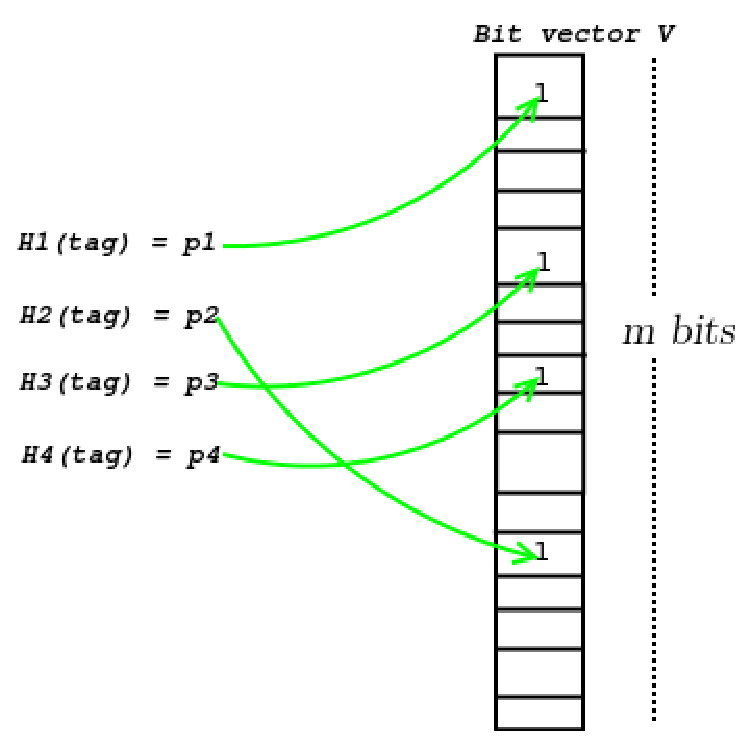
\includegraphics[scale=0.4]{bloom}
\end{figure}
\end{frame}

\begin{frame}[fragile] % Need to use the fragile option when verbatim is used in the slide
\frametitle{Index aggregation \& routing}
\begin{figure}
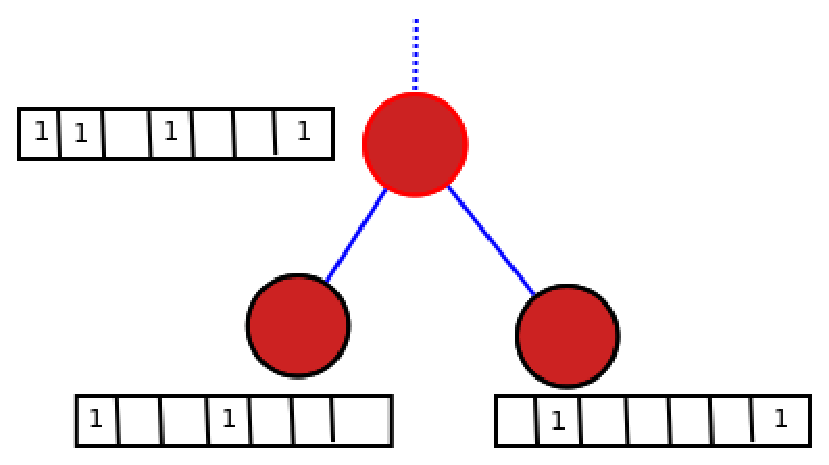
\includegraphics[scale=0.4]{d3}
\end{figure}
\end{frame}

\begin{frame}[fragile] % Need to use the fragile option when verbatim is used in the slide
\frametitle{Index aggregation \& routing}
\begin{figure}
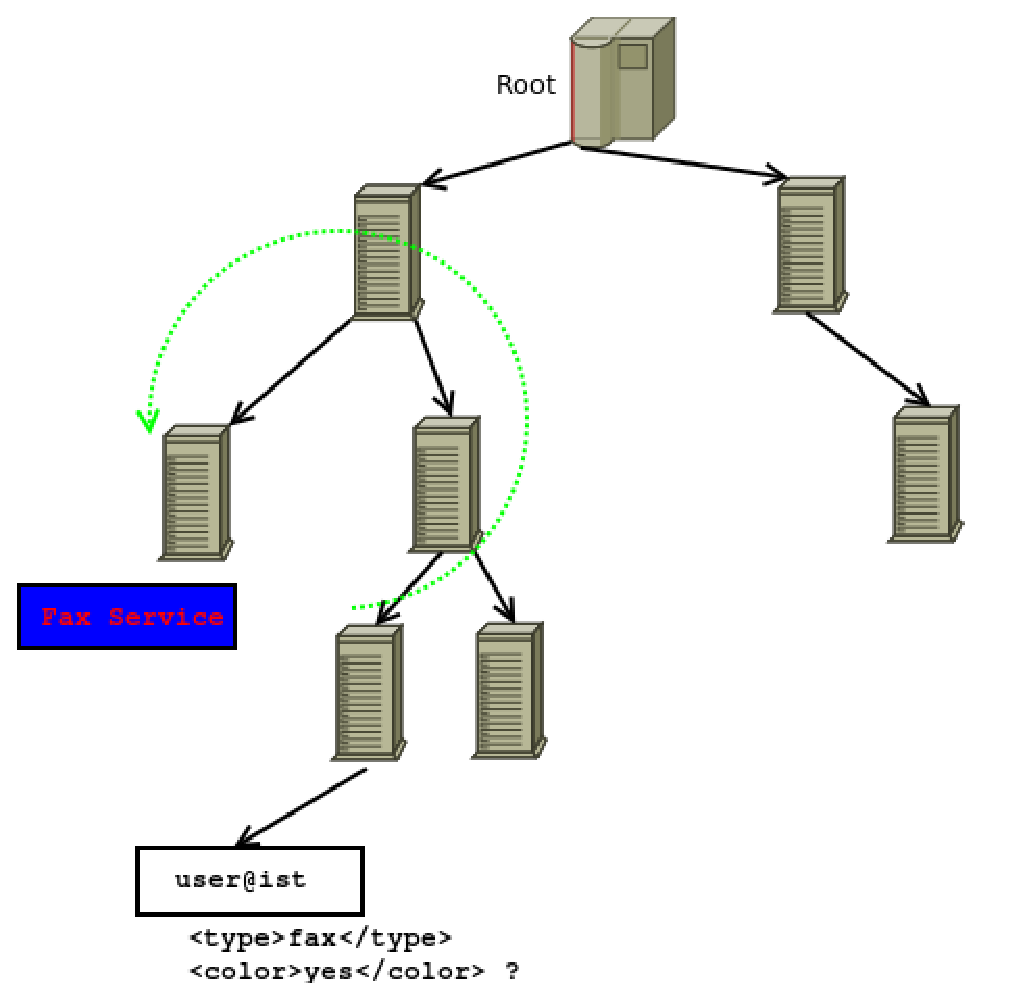
\includegraphics[scale=0.4]{d4}
\end{figure}
\end{frame}

%------------------------------------------------
\section{System Performance}
\begin{frame}[fragile] % Need to use the fragile option when verbatim is used in the slide
\frametitle{System Performance}
\begin{figure}
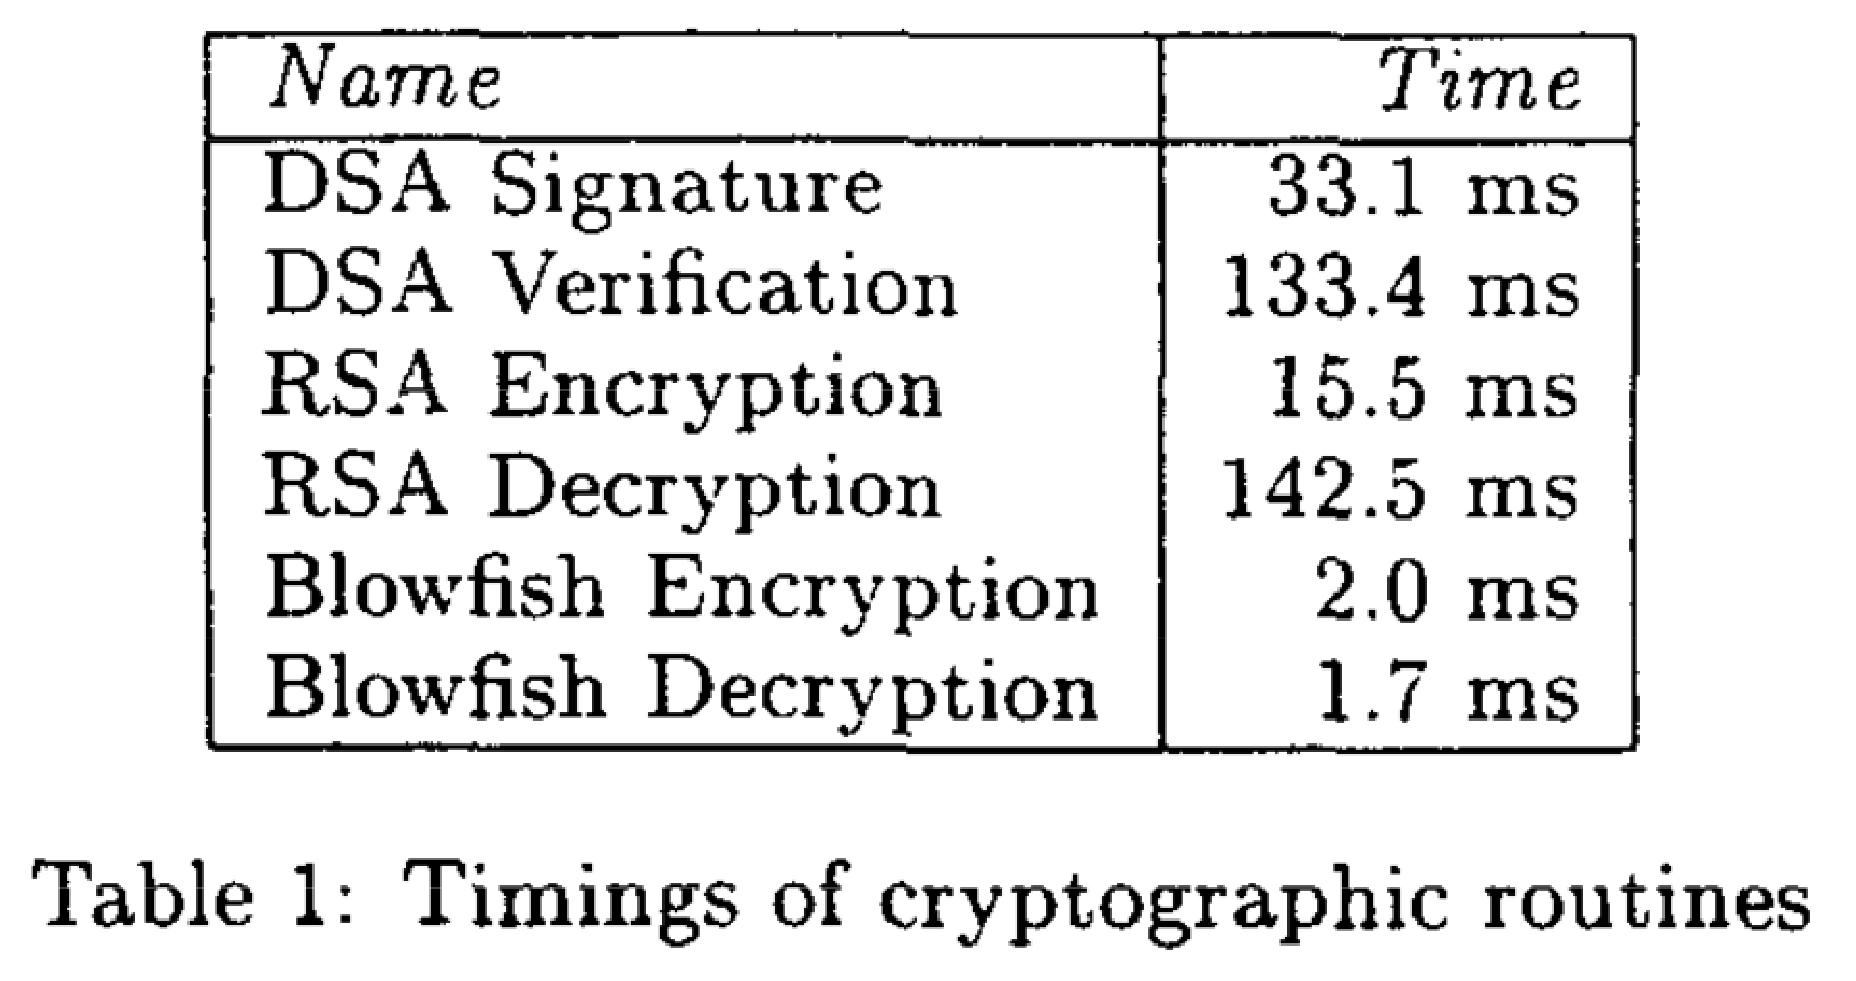
\includegraphics[scale=0.2]{t1}
\end{figure}
\end{frame}

\begin{frame}[fragile] % Need to use the fragile option when verbatim is used in the slide
\frametitle{System Performance}
\begin{figure}
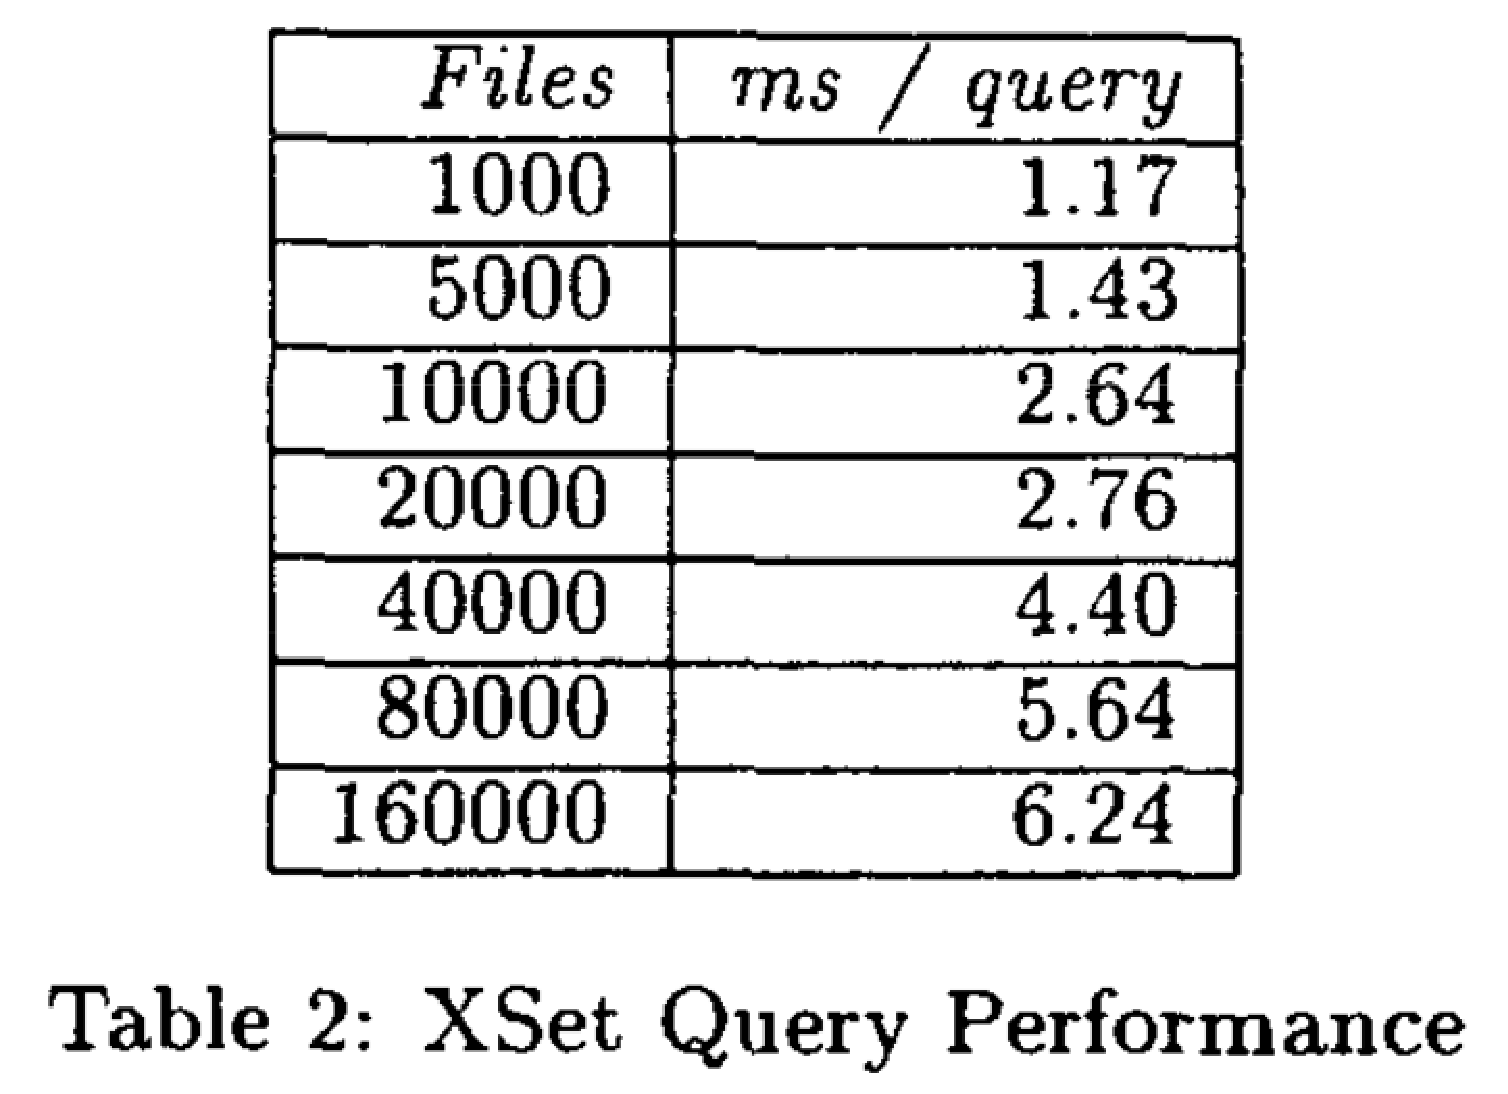
\includegraphics[scale=0.2]{t2}
\end{figure}
\end{frame}

\begin{frame}[fragile] % Need to use the fragile option when verbatim is used in the slide
\frametitle{System Performance}
\begin{figure}
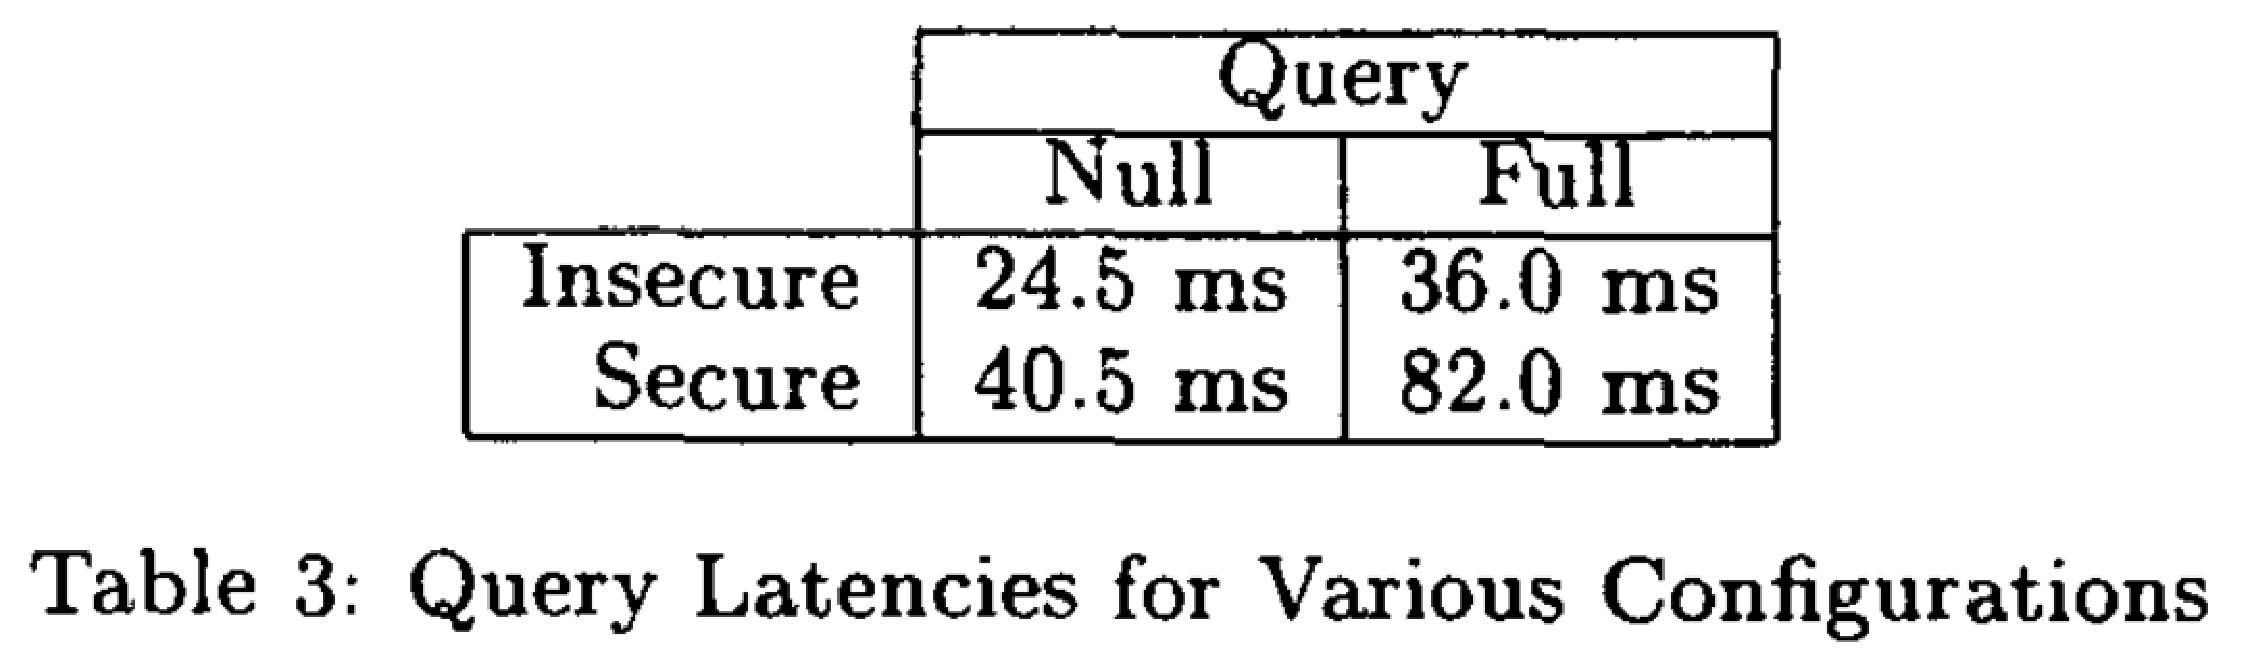
\includegraphics[scale=0.2]{t3}
\end{figure}
\end{frame}


\begin{frame}[fragile] % Need to use the fragile option when verbatim is used in the slide
\frametitle{System Performance}
\begin{figure}
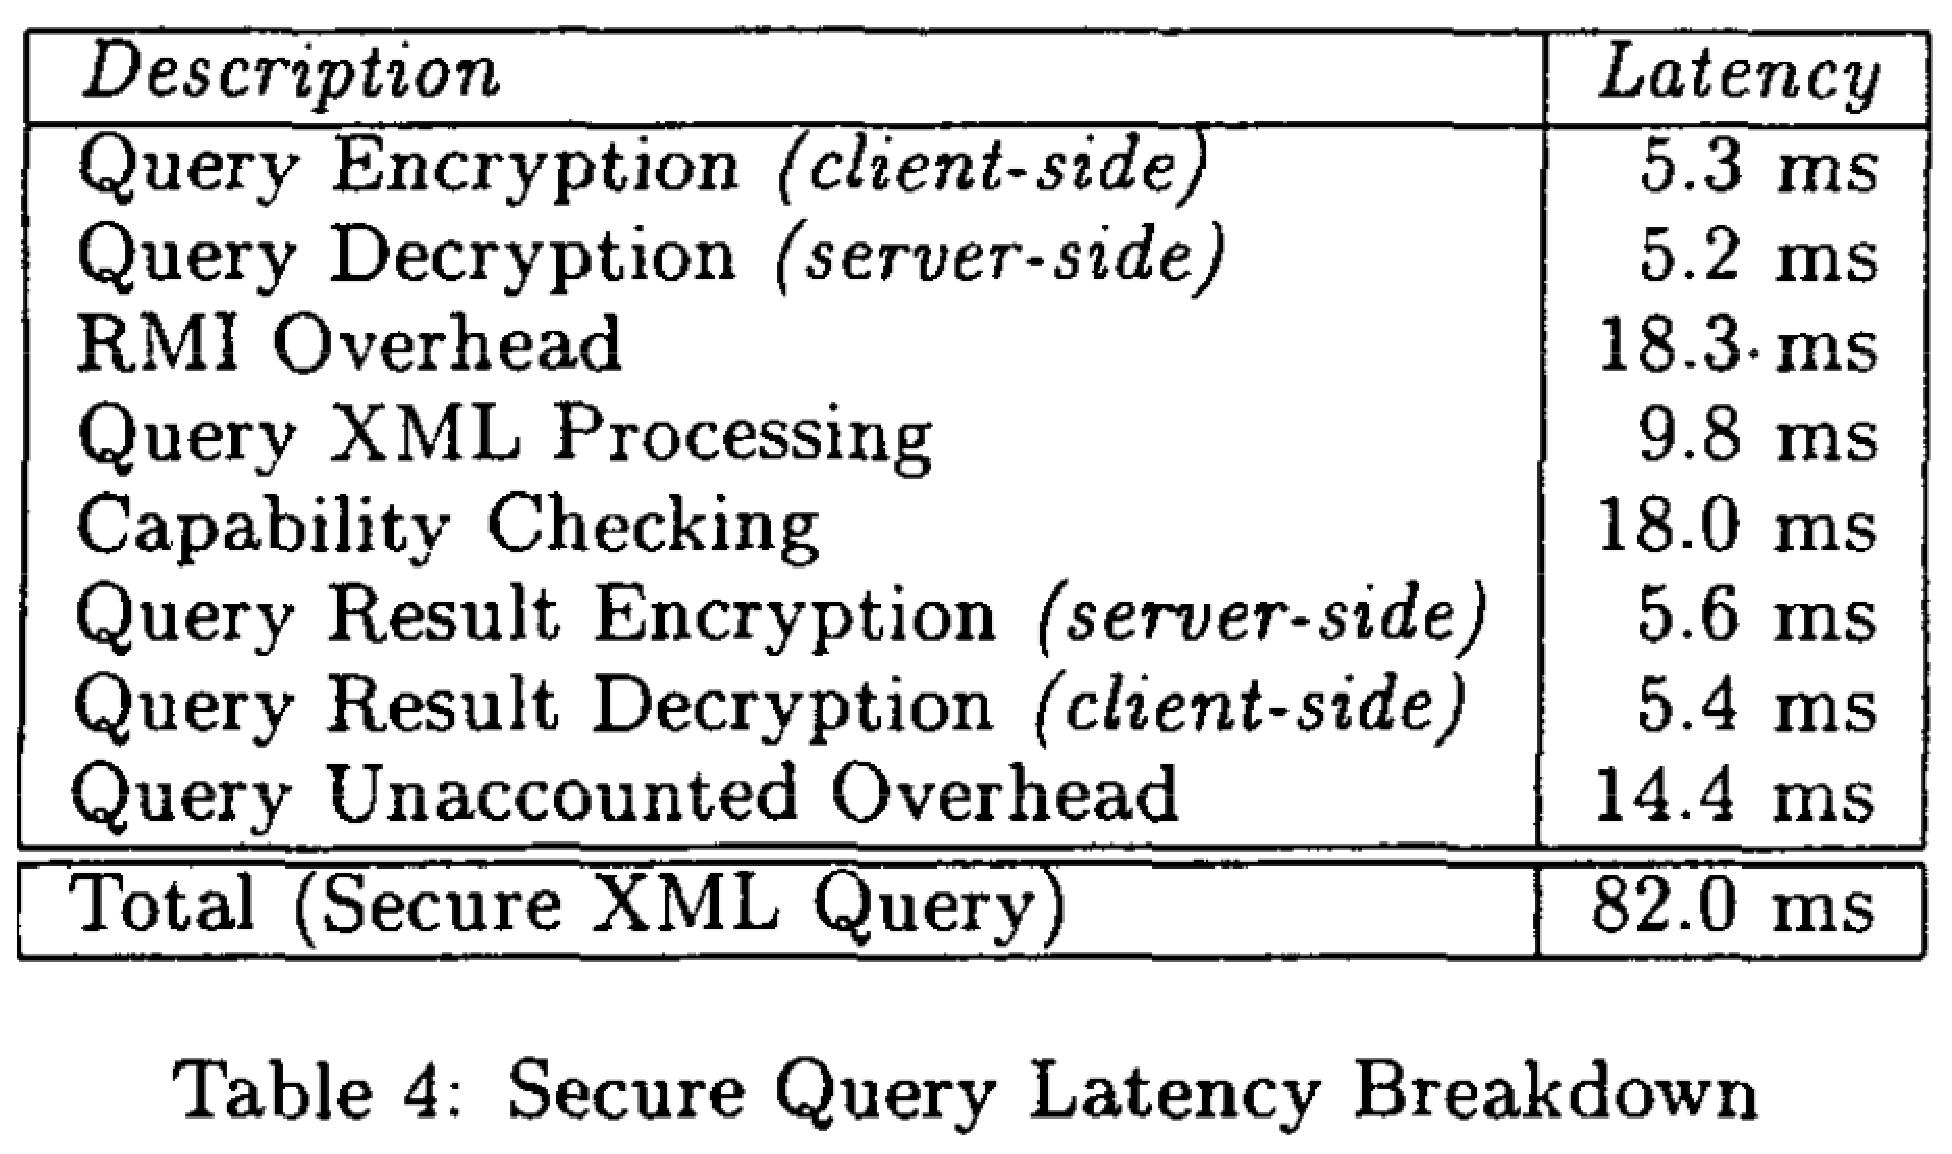
\includegraphics[scale=0.2]{t4}
\end{figure}
\end{frame}

\begin{frame}[fragile] % Need to use the fragile option when verbatim is used in the slide
\frametitle{Related Work}
\begin{itemize}
\item {\bf DNS \& Globe}
\item {\bf Condor Classads}
\item {\bf JINI}
\item {\bf Service Location Protocol}
\end{itemize}
\end{frame}


\section{Conclusion}
\begin{frame}[fragile] % Need to use the fragile option when verbatim is used in the slide
\frametitle{Conclusion}
Work still needed on: 
\begin{itemize}
\item {\bf Wide area implementation }
\item {\bf Benchmarking }
\item {\bf Ninja infrastructure necessary to evaluate}
\end{itemize}
\end{frame}


\begin{frame}
\Huge{\centerline{Questions ?}}
\end{frame}

%----------------------------------------------------------------------------------------

\end{document}
